\begin{figure}[H]
\centering
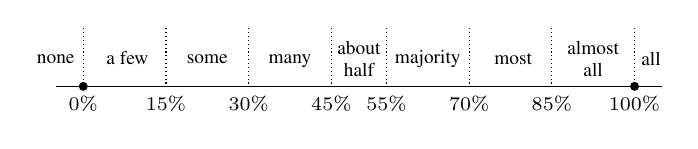
\begin{tikzpicture}[scale=0.070]
\draw[-] (-5,0) -- (105,0) ; %edit here for the axis
\foreach \x in {0,15,30,45,55,70,85,100} % edit here for the vertical lines
\draw[densely dotted, shift={(\x,0)},color=black] (0pt,300pt) -- (0pt,0pt);
\foreach \x in {0,15,30,45,55,70,85,100} % edit here for the numbers
\draw[shift={(\x,0)},color=black] (0pt,0pt) -- (0pt,-0pt) node[below] % xlabel and bottom half color
{\scriptsize$\x\%$};
\draw (0,0) circle[radius=20pt];
\fill (0,0) circle[radius=20pt];
\draw (100,0) circle[radius=20pt];
\fill (100,0) circle[radius=20pt];
\fontfamily{ptm}{
\node[align=center,font=\scriptsize] at (103,5) {all};
\node[align=center,font=\scriptsize] at (-5,5) {none};
\node[align=center,font=\scriptsize] at (8,5.2) {a few};
\node[align=center,font=\scriptsize] at (22.5,4.9) {some};
\node[align=center,font=\scriptsize] at (37.5,4.5) {many};
\node[align=center,font=\scriptsize] at (50,5) {about\\half};
\node[align=center,font=\scriptsize] at (62.5,4.9) {majority};
\node[align=center,font=\scriptsize] at (78,5) {most};
\node[align=center,font=\scriptsize] at (92.5,5) {almost\\all};
}
\end{tikzpicture}
 \caption{Terminology used to present relative frequency of themes.}
    \label{fig:terminology}
\end{figure}
